\documentclass[12pt,letterpaper]{report}
\usepackage{graphicx}
\usepackage{scrextend}
\usepackage{vmargin}
\usepackage[utf8]{inputenc}
\usepackage[spanish]{babel}
\usepackage{multicol}
\usepackage{amsmath, amsthm, amssymb, amsfonts}
\usepackage[usenames]{color}
\parindent=0mm
\pagestyle{empty}
\definecolor{miorange}{rgb}{0.91, 0.43, 0.0}
\begin{document}
\setmargins{2.5cm}      
{1.5cm}                     
{2cm}  
{24cm}                    
{10pt}                          
{1cm}                          
{0pt}                             
{2cm} 
\begin{minipage}{0.3\linewidth}
\today
\end{minipage}
\begin{flushright}
\vspace*{-0.75cm}
\begin{minipage}{0.8\linewidth}
\begin{flushright}
Examen de práctica- Matemáticas\\
Universidad Autónoma de Nuevo León
\end{flushright}
\end{minipage}
\end{flushright}
\begin{enumerate}
\item Tres cajas contienen, cada una, 12 kilogramos de carne de res, 18 de carne de cerdo y 24 de carne de pollo. La carne
de cada caja está contenida en bolsas del mismo tamaño y con la máxima cantidad de carne posible, ¿cuánto pesa
cada bolsa y cuántas hay por caja?
\item En el año 2000 el número de habitantes de una población fue de 1.8 millones, para el año siguiente su incremento
fue de 0.25 millones y para el tercer año aumentó 0.75 millones, ¿cuántos habitantes había al final del año 2002?
\item Simplifica las siguientes expresiones
\begin{itemize}
\item[a)] 
\begin{equation*}
\left( \frac{2^{-8}\cdot 3^5 \cdot 5^{-6}}{2^{-7}\cdot 3^6 \cdot 5^{-5}} \right)
\end{equation*}
\item[b)]
\begin{equation*}
\left( \frac{3^{-4}\cdot 5^{-1}}{3^2 \cdot 5^{-3}}\right)^{-\frac{1}{2}} \left( \frac{3^4\cdot 5^4}{3^2 \cdot 5^4}\right)^{-1}
\end{equation*} 
\item[c)]
\begin{equation*}
\left[\left(\frac{1}{2}\right)^2 \left(\frac{3}{5}\right)^2  \right]^2
\end{equation*}
\item[d)]
\begin{equation*}
\sqrt[3]{3^6 \cdot 5^3 }
\end{equation*}
\item[f)]
\begin{equation*}
\left(\sqrt[4]{9} \right)^4
\end{equation*}
\item[g)]
\begin{equation*}
5\sqrt{8}-\sqrt{27}-\sqrt{32}+3\sqrt{3}+\sqrt{2}
\end{equation*}
\item[h)]
\begin{equation*}
\sqrt{200}+\sqrt{50}-\sqrt{98}-\sqrt{338}
\end{equation*}
\end{itemize}
\item Un automóvil gasta 9 litros de gasolina cada 120 km. Si quedan en el depósito 6 litros, ¿cuántos kilómetros podrá
recorrer? 
\item Un grupo de 45 estudiantes de CONAMAT contrata un autobús para ir a un evento y calculan que cada uno debe pagar
\$50; finalmente sólo asisten 30 estudiantes, ¿cuánto deberá pagar cada uno?
\item Si 24 motocicletas repartidoras de pizzas gastan \$27,360 en gasolina durante 30 días trabajando 8 horas diarias,
¿cuánto dinero se deberá pagar por concepto de gasolina para 18 motocicletas que trabajan 10 horas diarias durante
6 meses? (considera meses de 30 días).
\item Para aprobar un examen de 60 reactivos, Mónica tiene que contestar correctamente 75\% de éste, ¿cuál es el mínimo
de preguntas que deberá contestar acertadamente para aprobarlo?
\item Dos ciudades M y N se encuentran a 640 km de distancia entre sí. A las 10 de la mañana de la ciudad M sale un
automóvil rumbo a la ciudad N, con una velocidad de 85
km/h, a la misma hora de N sale otro automóvil rumbo a M
con una velocidad de 75
km/h, ¿a qué hora se encontrarán y qué distancia ha recorrido cada uno?
\item Simplifica las siguientes expresiones
\begin{enumerate}
\item $4x-3x-2x$
\item $-3a^{m+5}+10x^{m+2}+2a^{m+5}-3x^{m+2}-8a^{m+5}$
\item $10a-7b+4a+5b-14a+3b$
\item
\begin{equation*}
\frac{5}{2}x^2-5xy+\frac{2}{3}y^2+\left(-\frac{1}{3}x^2+\frac{3}{2}xy-\frac{1}{4}y^2 \right)+\left(-2x^2+\frac{1}{2}xy-\frac{3}{4}y^2 \right)
\end{equation*}
\item
\begin{equation*}
\left(\frac{3}{2}x^5-\frac{1}{4}x^2-6x+\frac{2}{3} \right)- \left(\frac{1}{2}x^2-\frac{5}{2}x^2-\frac{2}{3}x-1 \right)
\end{equation*}
\item
\begin{equation*}
\frac{2}{3}a-\left[ -\frac{1}{5}b-\left(2a-\frac{3}{5}b\right)+\frac{2}{3}a \right]-\frac{1}{2}b
\end{equation*}
\item 
\begin{equation*}
\left(-\frac{3}{4}a^6b \right)\left(\frac{2}{3}a^2bc \right)\left( -\frac{1}{2}ac\right)\left( -2b^2c^2\right)
\end{equation*}
\item 
\begin{equation*}
\left(3x^{3a-1} \right)\left( -4x^{2a}y^{4a}\right)\left(-2x^{4a-1}y^{2a} \right)
\end{equation*}
\end{enumerate}
\item La distancia que hay de un punto hacia los extremos de un lago
son 145 y 215 metros, mientras que el ángulo entre las 2 visuales
es de 45$^{\circ}$. Calcula la distancia entre los extremos del lago.\\
\begin{center}
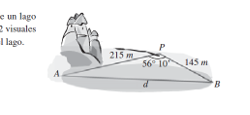
\includegraphics[scale=1]{images/imagen1.png}
\end{center}
\item En un paralelogramo que tiene un lado que mide 20.8 cm, su diagonal
mide 46.3 cm. Determina la longitud del otro lado si se sabe
que el ángulo entre la diagonal y el primer lado es de 30$^{\circ}$.
\begin{center}
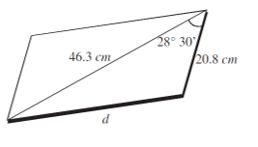
\includegraphics[scale=1]{images/imagen2.png}
\end{center}
\item Si con 12 botes de  $\frac{1}{2}$ l  de pintura cada uno se han pintado 90m de verja
de 80 cm de altura. Calcular cuántos botes de 2 l  de pintura serán necesarios
para pintar una verja similar de 120 cm de altura y 200 metros de longitud.
\item 11 obreros labran un campo rectangular de 220 m de largo y 48 de ancho en 6 días.
¿Cuántos obreros serán necesarios para labrar otro campo análogo de 300 m de
largo por 56 m de ancho en cinco días?
\item Al adquirir un vehículo cuyo precio es de 8800, nos hacen un descuento del 7.5\%.
¿Cuánto hay que pagar por el vehículo?
\item Resuleve la siguiente desigualdad cuadrática 
\begin{equation*}
x(3x+2)>(x+2)2
\end{equation*}
\item Un avión dispone de 32 asientos en clase A y de 50 asientos en clase B cuya venta supone un total de 14.600. Sin embargo, sólo sea han vendido 10 asientos en clase A y 40 en clase B, obteniendo un total de 7.000.
¿Cuál es precio de un asiento en cada clase?
\item Hallar un número de dos cifras que cumpla:
\begin{itemize}
\item La segunda cifra es el doble de la primera
\item La suma de las cifras es 12.
\end{itemize}
\item Con una cuerda de 34 metros se puede dibujar un rectángulo (sin que sobre cuerda) cuya diagonal mide 13 metros.
Calcular cuánto mide la base y la altura de dicho rectángulo.
\item Una urna tiene ocho bolas rojas, 5 amarilla y siete verdes. Si se extrae una
bola al azar calcular la probabilidad de:
\begin{itemize}
\item Sea roja.
\item  Sea verde.
\item  Sea amarilla.
\item  No sea roja.
\item  No sea amarilla.
\end{itemize}
\item Con las cifras 2, 2, 2, 3, 3, 3, 3, 4, 4;
¿Cuántos números de nueve cifras se pueden formar?
\item Se ordenan en una fila 5 bolas rojas, 2 bolas blancas y 3 bolas azules.
Si las bolas de igual color no se distinguen entre sí.
¿De cuántas formas posibles pueden ordenarse?
\end{enumerate}
\end{document}